\scanpage{36}
\[
g=\exp f\qquad f'=\varphi=\unsure{\psi|\Psi}^{1/2}
\]
\[
g'=(\exp f)f'\deleted{=\unsure{(\exp f)\varphi}}
\]
\[
g''=(\exp f)f'^2+(\exp f)f''=(\exp f)(f'^2+f'')
\]
\[
\begin{aligned}
g'''&=(\exp f)f'(f'^2+f'')+(\exp f)(2f'f''+f''')\\
&=(\exp f)(f'^3+3f'f''+f''')
\end{aligned}
\]
\[
\frac{g'''}{g'}=f'^2+3f''+\frac{f'''}{f'}
\]
\[
\frac{g''}{g'}=f'+\frac{f''}{f'}\qquad
\left(\frac{g''}{g'}\right)^2=f'^2+\left(\frac{f''}{f'}\right)^2+2f''
\]
\[
\begin{aligned}
-2\frac{g'''}{g'}+3\left(\frac{g''}{g'}\right)^2
&=\uline{-2f'^2}-\deleted{6f''}-2\frac{f'''}{f'}\\
&\quad+\uline{3f'^2}+3\left(\frac{f''}{f'}\right)^2+\deleted{6f''}\\
&=-2\frac{f'''}{f'}+3\left(\frac{f''}{f'}\right)^2+\deleted{\unsure{3}}f'^2
\end{aligned}
\]
\[
G(t,\exp f)=G(t,f)+3(df)^2
\]
\[
\begin{array}{c}
\Vert\\
-c_t+c_{\exp f}=-c_t+c_f+3(df)^2
\end{array}
\]
\[
\boxed{c_{\exp f}=c_f+\deleted{\unsure{3}}df^2}
\]
\[
c_{\exp f}=c_f+\deleted{\unsure{3}}df^2=c_f+\omega^{\unsure{\otimes2|2}}.
\]
\[
\begin{array}{l}
\varphi=\exp t\\
\varphi'=\exp t\\
\varphi''=\exp t\\
\varphi^{\unsure{'''}}=\exp t
\end{array}
\qquad
\left(-2\frac{\varphi'''}{\varphi'}+3\left(\frac{\varphi''}{\varphi'}\right)^2\right)dt^2=dt^2
\]
\[
c_f+\unsure{\omega^2|\infty}
\]

\margin{\figure{\begin{tikzpicture}[x=1cm,y=1cm]
\node (formula) at (0,1.2) {$\deleted{\unsure{C}}G(z,f)\deleted{\unsure{d}}=\left(-\unsure{2}\frac{f'''}{f'}+3\left(\frac{f''}{f'}\right)^2\right)dz^2$};
\node (note) at (-2,-.2) {\shortstack{\unsure{invariant} \unsure{pour} $\pi$\\\deleted{\unsure{automorphismes|homomorphismes}}\\\unsure{hyperboliques}}};
\draw (-4,.45) .. controls (-4.6,-.25) and (-3.8,-.9) .. (-2.1,-.85) .. controls (-.2,-.9) and (.3,.35) .. (-1,.45) -- cycle;
\draw[->] (-3.6,.45) .. controls (-3.2,.6) and (-3.1,.8) .. (-3.1,1);
\draw (-.8,.8) .. controls (-.4,.55) and (2,.65) .. (2.6,.75);
\node at (2,-.1) {$\dfrac{df}{dz}$};
\node[right] at (2.7,-.1) {\shortstack{forme inv. par\\$\pi$}};
\end{tikzpicture}}}

\margin{$G(f,z)\deleted{\unsure{df^2}}=0$}
\margin{\figure{\begin{tikzpicture}
\node at (0,0) {$\dfrac{d^3z}{df^3}$};
\draw (.4,.05) .. controls (.65,.12) and (1.4,.1) .. (1.7,.05);
\end{tikzpicture}}}
\margin{$G(f,z)=0$}
\margin{$G(z,f)=$}
\margin{$\begin{array}{c}
\unsure{\gamma}.G(z,f)\\
\Vert\\
G(\unsure{\gamma}.z,\unsure{\gamma}.f)\\
\Vert\\
G(\unsure{\gamma}z,f)\\
\Vert\\
G(z,f)
\end{array}$}
\figure{\begin{tikzpicture}\draw (0,0)--(0,1.4);\draw (.17,.05)--(.17,1.3);\end{tikzpicture}}
\margin{35}
